\chapter{Optical Detector Applications to measuring the active brain}
\label{ch:detectors}
The most precise method for measuring brain temperature is to use a thermocouple probe placed in direct contact with the tissue.  The disadvantage of this method and the reason it  can not be used in humans is because it is invasive and damaging.  Thus, an optical method would be ideal since it is non-invasive and non-damaging.  Currently, there does not exist a method for accurately measuring the temperature of brain tissue optically.  However, other optical measurements methods could be used in conjunction with a temperature model (such as the one proposed here) to calculate the temperature.  The possible application of functional Near-Infrared Spectroscopy (fNIRS) and its possible use in brain temperature calculations is discussed along with the limitations of a direct measurement technique such as a thermal imaging camera.
  
\section{{F}unctional {N}ear-{I}nfrared {fNIR} Spectroscopy}
% detector applicaitons to improving fNIR
\begin{figure}[tb]
  \begin{center}
    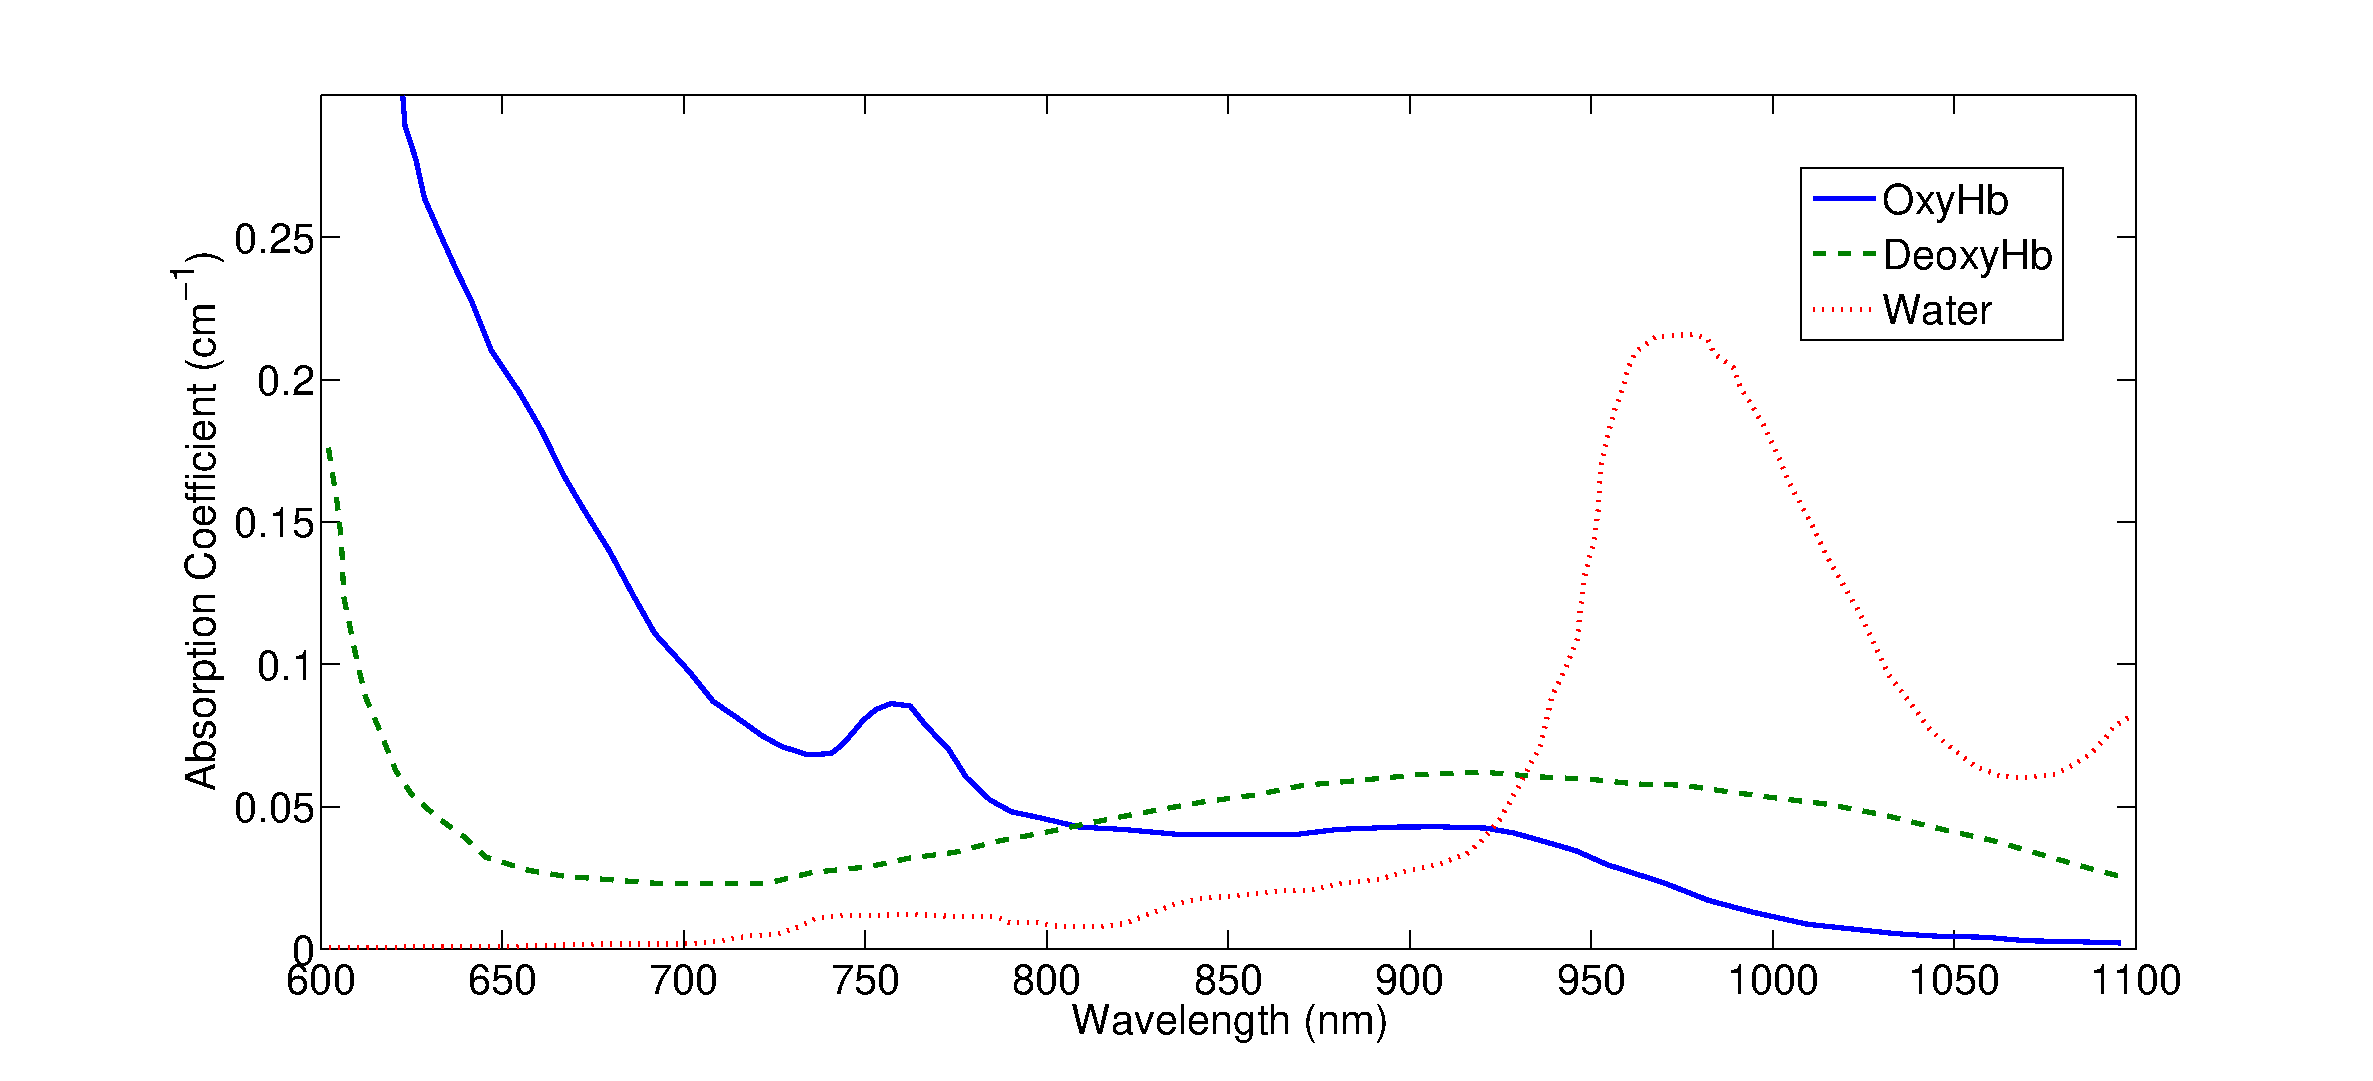
\includegraphics{AbsorptionData}
    \caption[Absorption spectra of water, deoxyhemoglobin and oxyhemoblogin]{\label{fig:fnirabsorption} Absorption spectra of water~\citet{cope}, oxyHb and deoxyHb~\citet{horecker}.}
  \end{center}
\end{figure}
\begin{table*}[tb]
  \begin{tabular*}{\linewidth}{lp{5cm}p{5cm}}
    \toprule
                         & fMRI             & fNIR            \\
    \midrule
    Spatial Resolution   & 8--27 mm$^3$  & $\sim$ 1--10 cm$^3$ \\
    Temporal Resolution  & 1--2 s        & $\sim$ 10$^{-3}$ s \\
    Measurement Parameter& blood volume, flow, and O$_2$ metabolism & oxyHb and deoxyHb concentrations \\
    Motion               & Must Remain Stationary & Small movements OK \\
    Penetration          & Whole-head    & outer 2--4 mm of brain tissue \\
    \bottomrule
  \end{tabular*}
  \caption[Comparison of fMRI and fNIR]{\label{tbl:comaparemethods}Comparison of the capabilities and limitations of fMRI and fNIR techniques.  Compiled from~\citet{bunce2006,elliott}.}
\end{table*}

As discussed in~\cref{ch:introduction}, changes in tissue activity can be detected by measuring the change in blood oxygenation levels.  Functional Magnetic Resonance Imaging (fMRI) is one technique for accomplishing this (the BOLD signal), but other techniques exist.  

Blood oxygenation can be determined by measuring the relative concentrations of oxyhemoglobin (oxyHb) and deoxyhemoglobin (deoxyHb).  Since oxyHb and deoxyHb have different absorption spectra (\cref{fig:fnirabsorption}), it is possible to determine this through optical techniques.  Functional Near-Infrared Spectroscopy is a technique which utilizes two or more spectral bands in order to determine blood oxygenation.  It has a high temporal resolution (millisecond), a low spatial resolution ($\sim$ 1~cm$^3$) compared to fMRI (as low as 1 mm$^3$), and is limited to only imaging the outer cortex (2--4 mm)~\citep{bunce2006}. A comparison of fMRI and fNIR is presented in~\cref{tbl:comaparemethods}.

fNIRS works by utilizing an array of near-infrared detectors and emitters (typically spaced 2--3 cm apart) placed in contact with the skin~\citep{villringer1997,izzetoglu2004}.  The exact spacing determines the depth the light is detected from.  As shown in~\cref{fig:fnirpenetration}, the closer the spacing, the higher the resolution but at the expense of lower penetration.  Conversely, in order to detect light passing through deeper tissue, a wider spacing is used which reduces the resolution.  The exact wavelengths used vary, but all lie within an optical window between 700--1000~nm~\citep{villringer1997} where absorption of near-infrared photons by tissue is low~(\cref{fig:fnirabsorption}).

\begin{figure}[tb]
  \centering
  \includegraphics{fnir-penetration}
  \caption[Penetration by fNIR]{\label{fig:fnirpenetration}Penetration depth of a fNIR detector as a function of the distance between the NIR LED emitter and detector.  Modified after~\citep{head2010}}
\end{figure}

Three techniques are used to illuminate the tissue: (i)~time domain (or time resolved spectroscopy, TRS), (ii)~frequency domain and, (iii)~continuous wave illumination~\citep{izzetoglu2004}.  In TRS, short pulses of light are incident on the tissue and the temporal distribution of photons in measured.  In frequency domain spectroscopy, the amplitude of the indecent light is modulated at a high frequency (10--100~MHz) and the phase shift and amplitude decay of the detected light is compared to the incident light~\citep{boas2002}. In continuous wave illumination, the incident light is not modulated so the detected light can only be compared for amplitude attenuation~\citep{izzetoglu2004}.

All of the techniques use a modified version of the Beer-Lambert Law~(\cref{eq:beerlambert})~\citep{cope}.  
\begin{equation}
  \label{eq:modifiedbeerlamber}
  I = G I_0 e^{-(\alpha_{deoxyHb}C_{deoxyHb}+\alpha_{oxyHb}C_{oxyHb})L} 
\end{equation}
where G is a factor to adjust for the measurement geometry, $I_0$ is in the incident light intensity, $\alpha_{oxyHb}$ and $\alpha_{deoxyHb}$ are the molar extinction coefficients for oxyHb and deoxyHb, $C_{oxyHb}$ and $C_{deoxyHb}$ are the chromophore concentrations for oxy-Hb and deoxy-Hb, and L is the path length~\citep{izzetoglu2004}.  By comparing a baseline measurement~($I_b$) with a new measurement~($I$), the optical density can be determined~\citep{izzetoglu2004}
\begin{equation}
  \Delta OD = \log \frac{I_b}{I} = \alpha_{deoxyHb} \Delta C_{deoxyHb}+\alpha_{oxyHb} \Delta C_{oxyHb}
\end{equation}
As discussed in~\citet{izzetoglu2004}, at least two wavelengths are utilized in the spectral window (700--1000~nm) in order to determine the change in concentration of chromophores $\Delta C_{deoxyHb}$ and $\Delta C_{oxyHb}$.  With these values, the oxygenation and total blood volume can be determined:
\begin{align}
  \label{eq:o2bloodvolume}
  Oxygenation\ &= \Delta C_{HBO2} - \Delta C_{HB} \nonumber \\
  Blood\ Volume\ &= \Delta C_{HBO2} + \Delta C_{HB} 
\end{align}
Using this method to experimentally measure the blood oxygenation while measuring the fMRI BOLD response could be used to better refine the current model for calculating the metabolism and blood flow from the BOLD response.

While fNIRS does not provide as spatially-precise a measurement as fMRI, it should be possible to modify the existing model for calculating temperature from the BOLD response to use fNIR data. This would be advantageous because fNIRS systems are cheaper and less disruptive than fMRI systems, meaning they can be used with a wider range of patients (children and the elderly).  For this reason, developing a model which uses fNIRS data should be considered in future research.

\section{Thermal Imaging}
\FloatBarrier

The primary challenge in brain temperature research is making experimental measurements of brain temperature.  The most accurate modality is to use a thermocouple probe, but since this is invasive and causes tissue damage, it is not possible to use this technique with human subjects.  For this reason, a non-invasive technique such as a thermal imaging camera is appealing.  Unfortunately, this technique is limited by the high absorption of mid-infrared photons by water.

Light absorption by a material is modeled using the Beer-Lambert law
\begin{equation}
  I = I_0 e^{-\alpha (\lambda) x} \label{eq:beerlambert}
\end{equation}
where $I$ is the intensity at a depth $x$ remaining from light with an incident intensity $I_0$ in a material with absorption coefficient $\alpha$.  The point at which the intensity has decayed to 1/$e$ (about 37\%) of the incident intensity is called the penetration depth, $\delta_{p}$
\begin{equation}
  \delta_p = \frac{1}{\alpha (\lambda)} \label{eq:penetrationdepth}
\end{equation}
This equation can be used along with the black body spectrum at tissue temperatures (\cref{fig:blackbody}) we can estimate the penetration depth of mid-infrared photons passing through water.

\begin{figure}[tb]
  \centering
  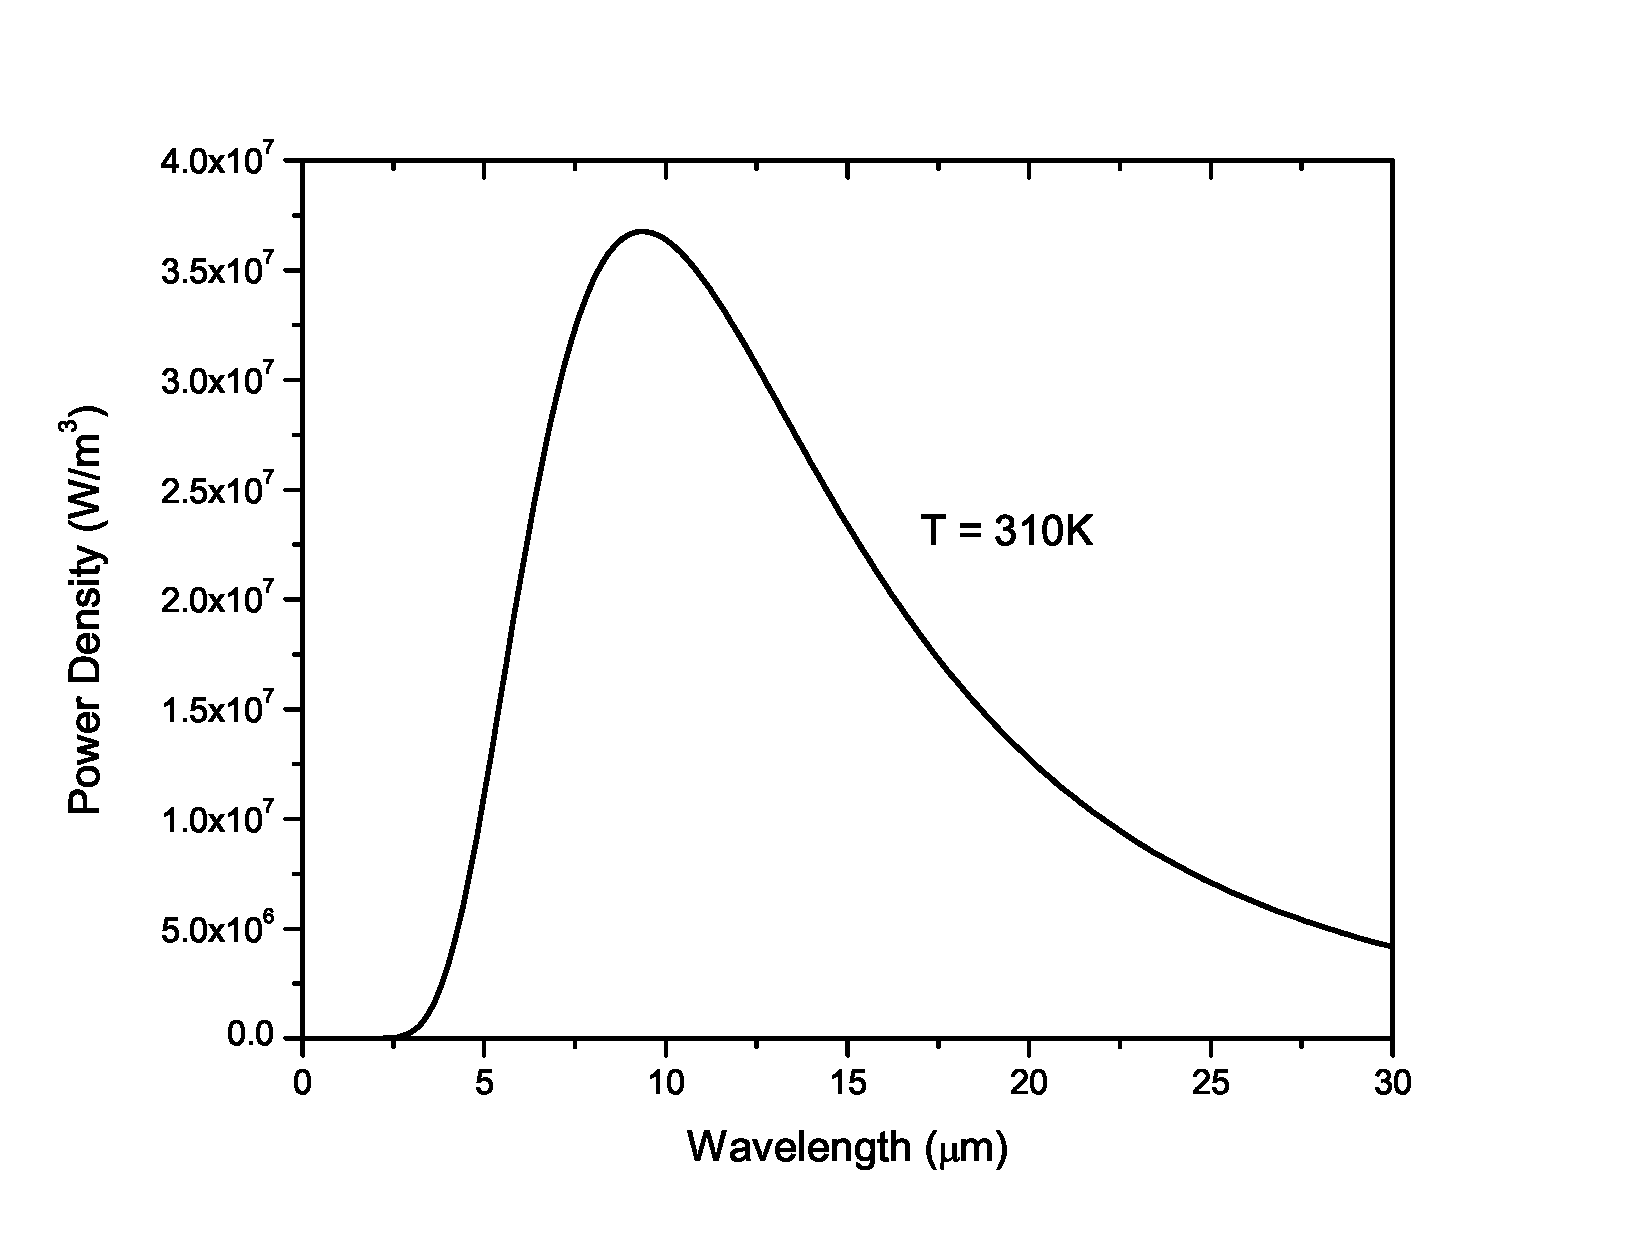
\includegraphics{blackbody310K}
  \caption[Black-body Spectrum at 310 K]{\label{fig:blackbody}Black-body spectrum at 310 K calculated using Planck's Law.}
\end{figure}
\begin{figure}[tb]
  \centering
  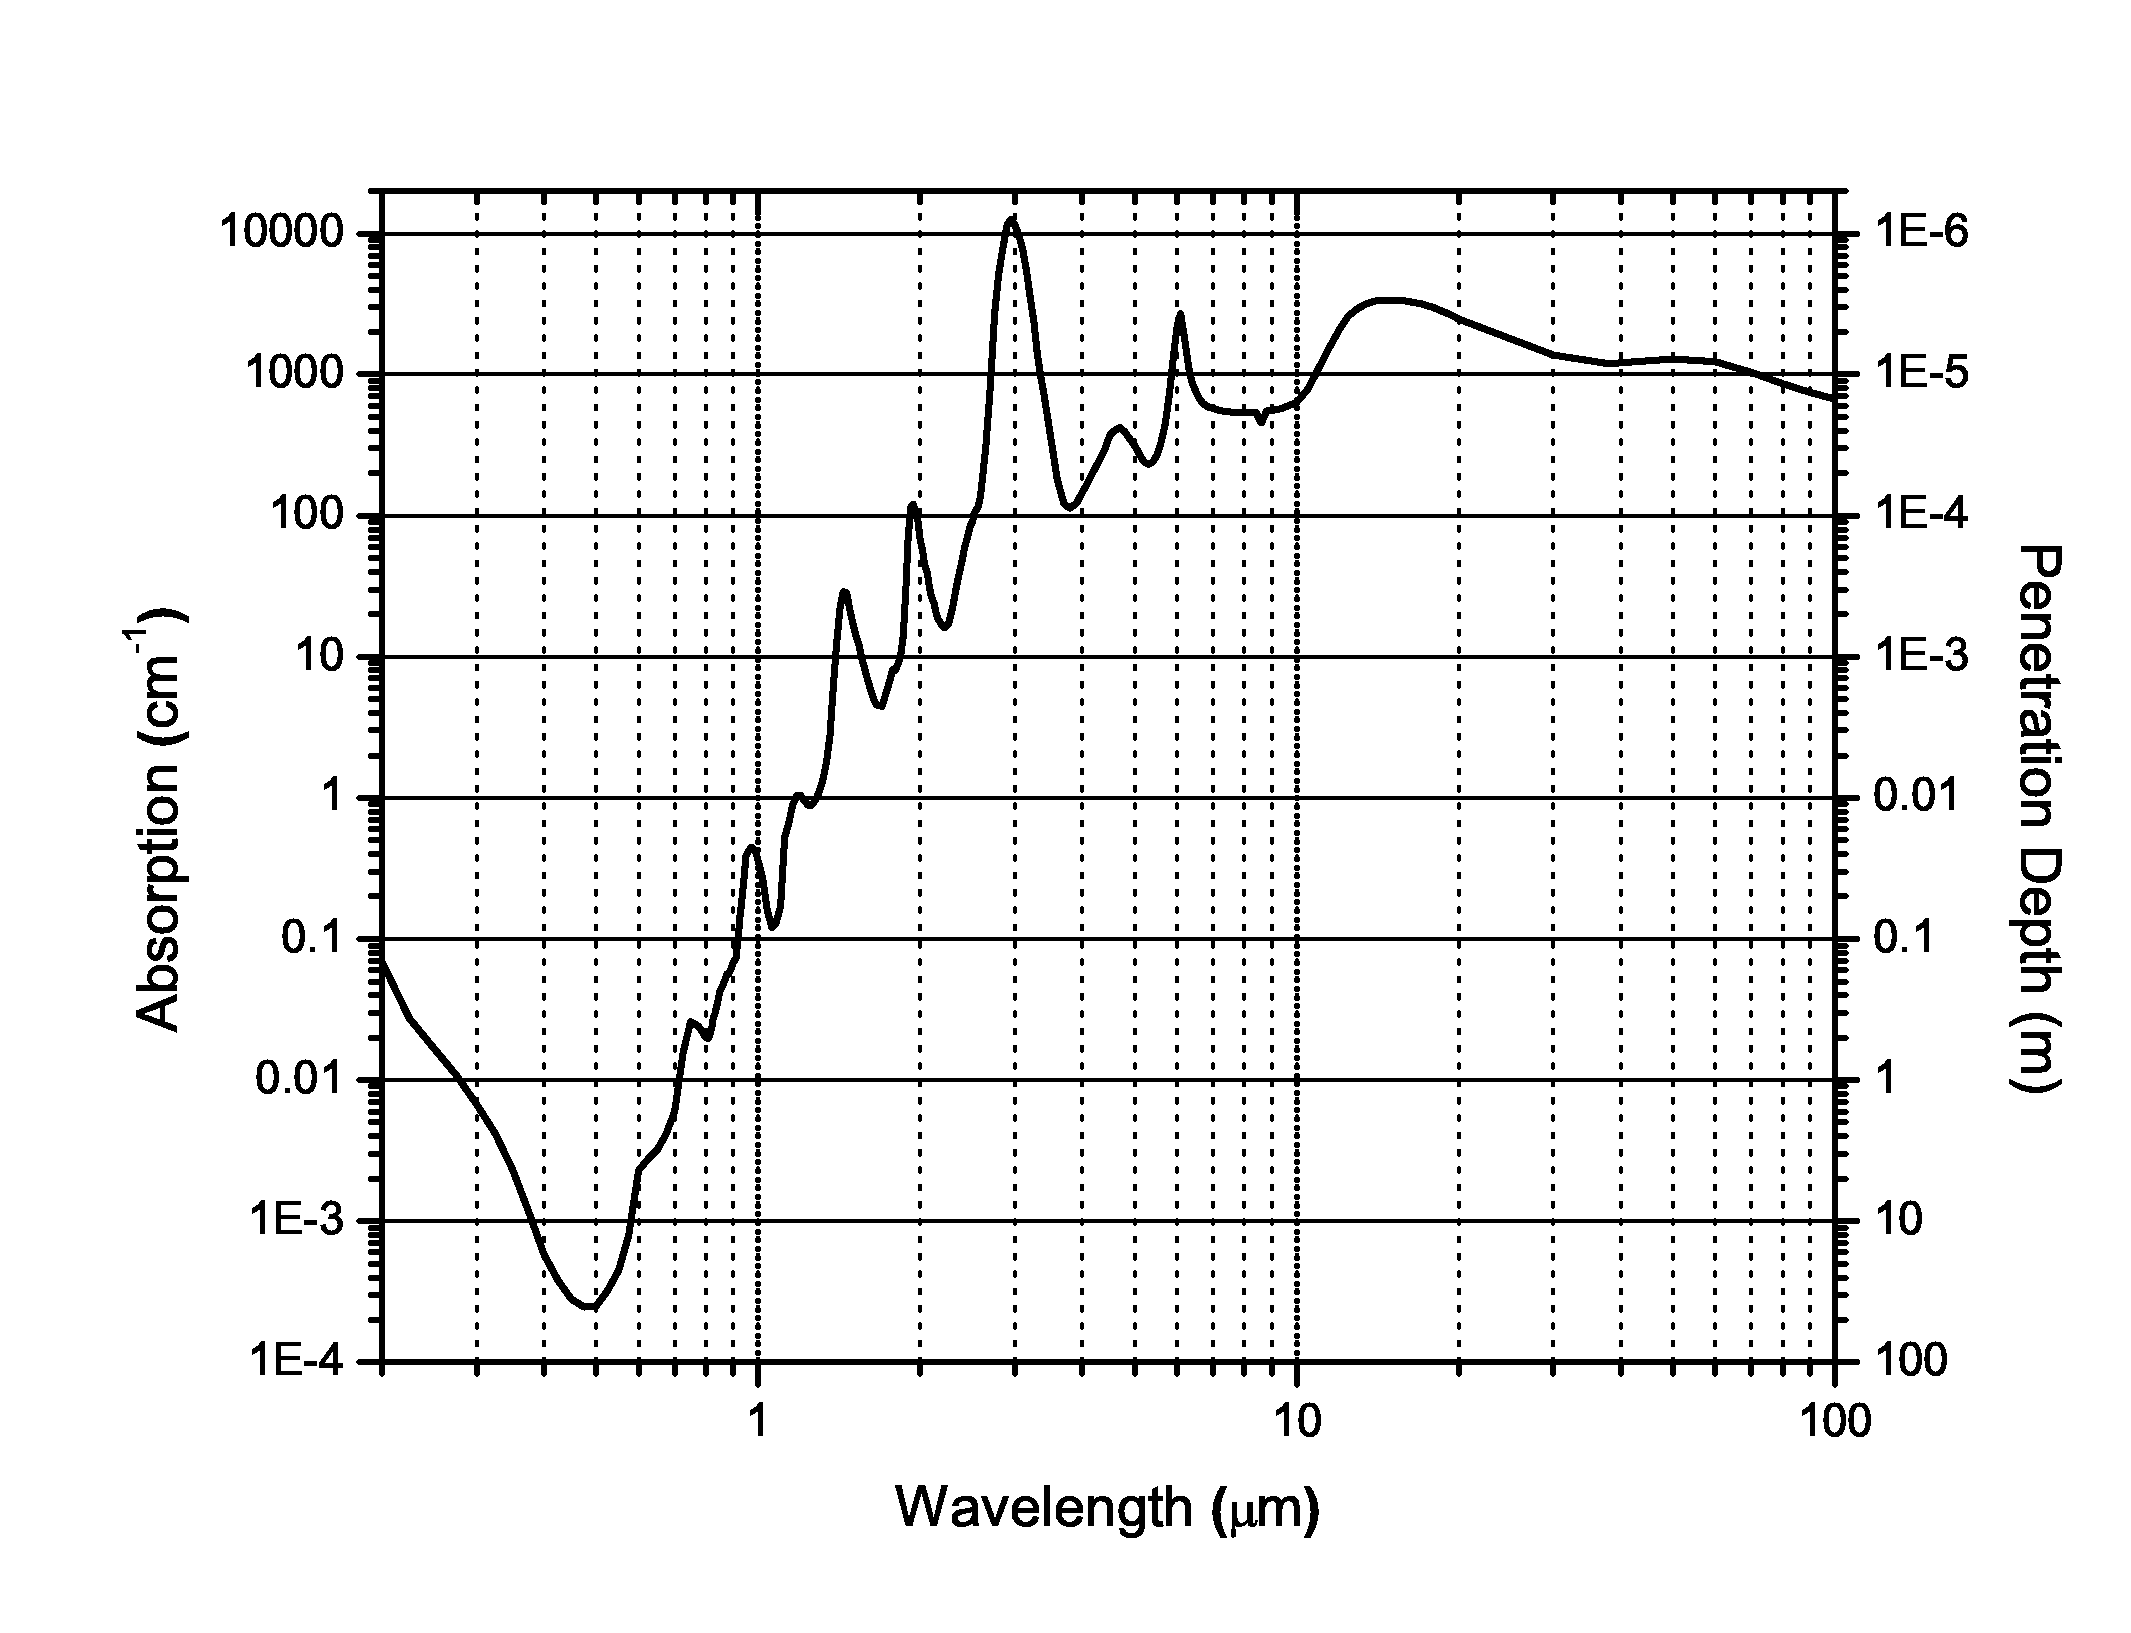
\includegraphics{water-wide-band}
  \caption[Wide-band absorption spectra of water]{\label{fig:waterabs}The absorptions spectra of water from UV to far-infrared.  Modified from~\citet{hale73}.}
\end{figure}

Wien's Displacement Law is a solution to Planck's law for the peak light emission wavelength:
\begin{align}
  \lambda_{max} &= \frac{b}{T} \label{eq:wienslaw} \\
  b &= 2.897\,7721 * 10^{-3} \mbox{ K m} \nonumber
\end{align}
where $b$ is Wien's displacement constant and T is the temperature in kelvin.  For $T=310$~K ($T=37\degree$~C), Wien's law yields a peak black-body emission wavelength of 9.35~\textmu m.  

Using~\cref{fig:waterabs} to find the absorption coefficient of approximately 700~cm$^{-1}$.  With the absorption coefficient, the penetration depth (\cref{eq:penetrationdepth}) is approximately 0.14~\textmu m.  This depth is roughly five orders of magnitude smaller than the distance from the surface of the brain to the surface of the head.  Thus, it can be assumed that a thermal imaging camera is unable to image photons coming from the brain.

When a thermal imaging camera is used, the photons collected come from the skin of the head rather than from any deeper tissues, thus it is not a viable form of brain activity detection unless direct line of sight to the brain is available (such as in an open skull surgery).  In this case, the temperature sensitivity of currently available cameras is greater than 14~mK~\citep{flir,ici} so it would be limited to only the most extreme of excitations.  As a comparison, the finger-tapping task discussed in the results section (\cref{sec:experimentalresults}) only induced a peak temperature change of 25~mK after tapping for about 170~seconds.  Detection of this activity would be at the limits of a thermal imaging camera.

While its applications to detecting brain activity are limited, thermal cameras could find use in the operating room.  It has been found that inducing mild hypothermia in patients being treated for cerebral ischemia improves the clinical outcome~\citep{maher1993}. The same treatment has been shown to improve the outcome of patients who have experienced a stroke~\citep{krieger2001}. Currently, the temperature of the brain is inferred from the core body temperature (which is monitored via an invasive thermistor catheter). If it is possible to directly image the brain (i.e. during surgery) then the hypothermia treatment can be better monitored through a thermal imaging camera.  This would be especially useful since conductive and radiative heat loss to the air from an exposed brain could reduce how tightly regulated the brain temperature is by the arterial blood temperature.

Optical detectors face many challenges working with biological tissue, the worst being infrared light absorption by water. fNIRS works within an optical window in the water absorption in order to measure changes in blood oxygenation, while thermal imaging is limited to measuring the temperature of tissue it has direct line of sight with because of the high absorption of water in the operating window. Despite their limitations, both of these techniques could be used in future studies to improve our understanding of brain temperature dynamics.